\documentclass[12pt,a4paper]{article}
\usepackage[slovene]{babel}
\usepackage{amsmath}
\usepackage{amsfonts}
\usepackage{amssymb}
\usepackage{graphicx}
\usepackage{lmodern}
\usepackage{hyperref}
\usepackage{xcolor}
\usepackage{adjustbox}
\usepackage{multirow}
\usepackage[left=2cm,right=2cm,top=2cm,bottom=2cm]{geometry}
\author{Tina Zwittnig 64200432}
\title{Poročilo 6. vaje pri predmetu OVS \\ Houghova preslikava}


\begin{document}
\maketitle
\pagebreak
\section{Najbolj izrazita premica}
Prvo smo poiskali najizrezitejše premice na sliki box1.png. Za parametre smo uporabili $\Delta \varphi = 4$, $\Delta r = 4$, $\sigma =0,5$, prag pa smo prav tako nastavili na 0,5. Največja vrednost v akumulatorju je 188. \\
\begin{figure}[h!]
  \begin{center}
    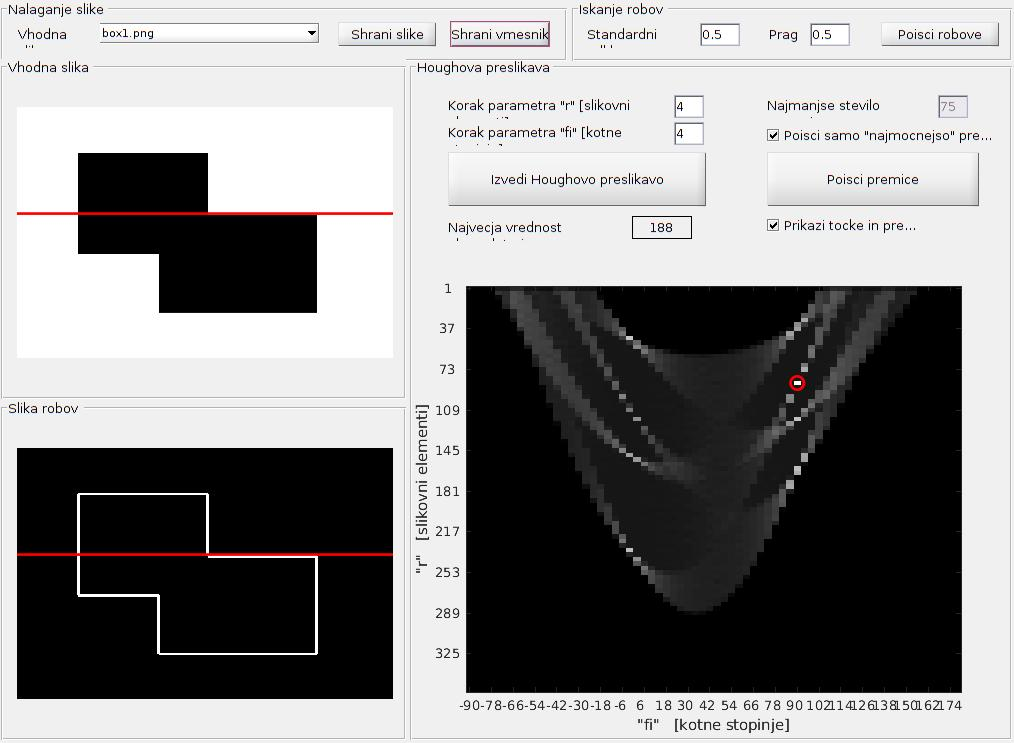
\includegraphics[scale = 0.3]{slika_4_uporabniski_vmesnik.jpg}
    \caption{Uporabniški vmesnik na sliki box1.png z poiskano najizrazitejšo premico}
    \label{fig:}
  \end{center}
\end{figure}\\
\begin{figure}[h!]
  \begin{center}
    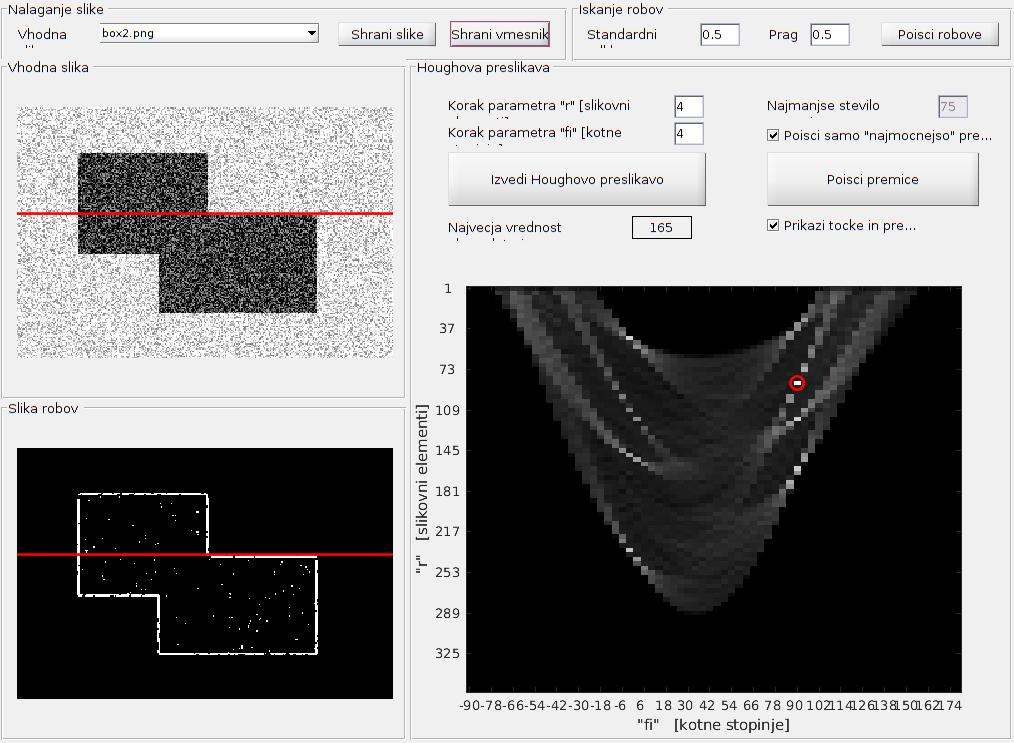
\includegraphics[scale = 0.3]{slika_4_uporabniski_vmesnikb.jpg}
    \caption{Uporabniški vmesnik na sliki box2.png z poiskano najizrazitejšo premico}
    \label{fig:}
  \end{center}
\end{figure}\\
\\
Postopek ponovimo na skiki box2.png. V tem primeru je največja vrednost v akumulatorju enaka 165.\\

Kot lahko vidimo postopek izbere enako najizrezitejšo premico. Iz tega lahko sklepamo, da če imamo na sliki kakšen šum, to ne vpliva bistveno na iskanje premice na sliki. Ko imamo prikazane robove lahko vidimo, da so na mestih nekoliko prekinjeni, vendar tudi to ne vpliva na iskanje premic. 
\section{Zmanjšana koraka $\Delta \varphi$ in $\Delta r$}
Ko manjšamo $\Delta \varphi$ in $\Delta r$ s tem večamo število vrednosti v akumulatorju. S tem izboljšujemo natančnost iskanja premic, saj pazimo, da so vrednosti dovolj \textgravedbl blizu \textacutedbl, ta ko ne povežemo dveh točk, ki ležita da drugih premicah, ampak le točki, ki sta na isti premici. Primerjava je lepo vidna, če za $\Delta \varphi = \Delta r = 10$ v primerjavi z $\Delta \varphi = \Delta r = 1$. 
\begin{figure}[h!]
  \begin{center}
    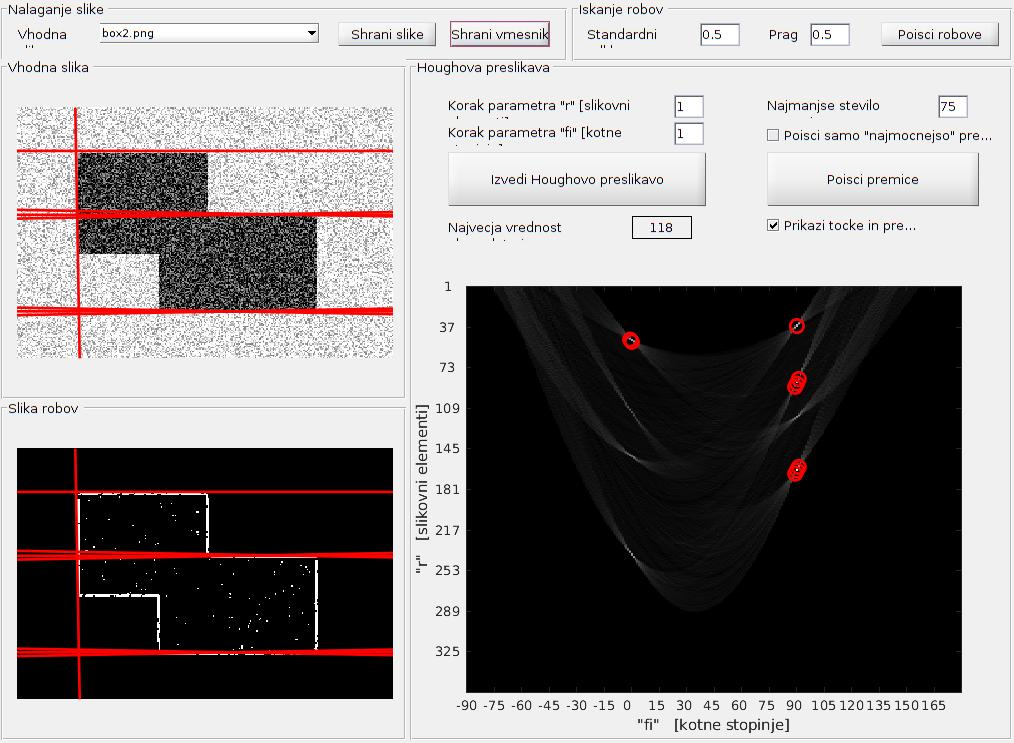
\includegraphics[scale = 0.3]{r1.jpg}
    \caption{najdene premice, če za parametre vzememo$\Delta \varphi = \Delta r = 1$ }
    \label{fig:}
  \end{center}
\end{figure}
\begin{figure}[h!]
  \begin{center}
    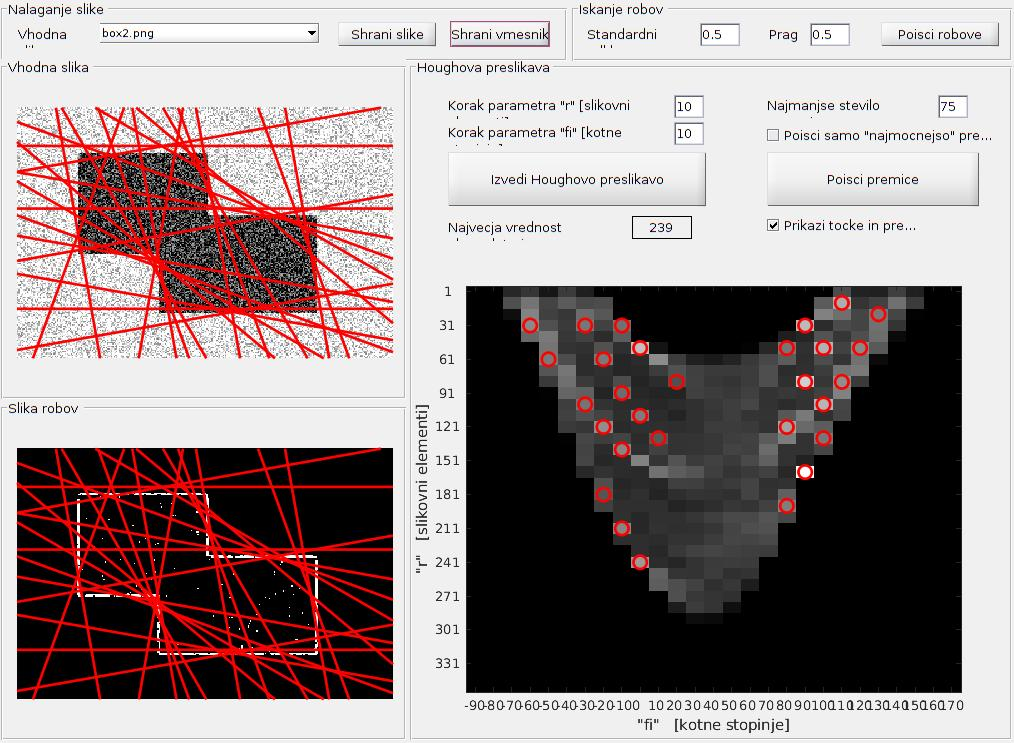
\includegraphics[scale = 0.3]{r10.jpg}
    \caption{najdene premice, če za parametre vzememo$\Delta \varphi = \Delta r = 10$}
    \label{fig:}
  \end{center}
\end{figure}
\pagebreak
\section{Natančnost določanja premic}
Na natačnost Hughove preslikave vpliva vhodna slika, kjer imamo že izrisane robove. Če robovi niso lepo zaznani bo tudi Hugova preslikava našla drugačne premice kot, če bi imela lepo določene robove.
Odvisna je tudi od  $\Delta \varphi, \Delta r$ In sicer, če manjšamo vrednosti, bo preslikava natančenjše našla premice. 
\section{Lastnosti Hughove preslikave}
 Če višamo število parametrov krivulje (da naprimer iščemo krožnico, hiperbolo...) računska zahtevnost raste. Kljub temu, je uporabna, ker če imamo prekinjene robove, preslikava še kar najde premice. Tudi če robovi niso zelo jasni lahko jih lahko z to preslikavo določimo.
 \section{Določanje centra}
 \subsection{Sobelova operatorja}
\begin{figure}[h!]
  \begin{center}
    \includegraphics[scale = 0.7]{operator.png}
    \caption{Prikaz amplitudne slike gradienta}
    \label{fig:}
  \end{center}
\end{figure}
\pagebreak
\subsection{Upragovanje}
\begin{figure}[h!]
  \begin{center}
    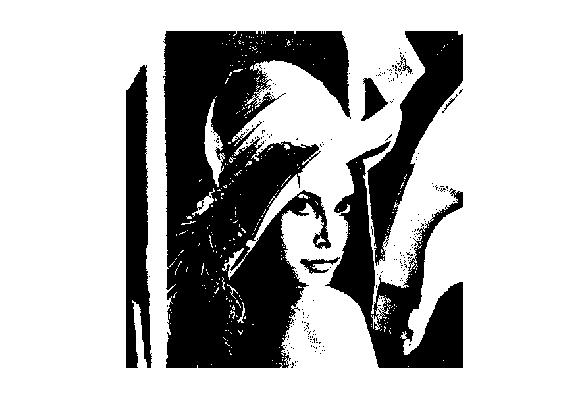
\includegraphics[scale = 0.7]{prag.png}
    \caption{Slika dobljena z upragovanjem, pri parametru 255/2}
    \label{fig:}
  \end{center}
\end{figure}
\pagebreak
\pagebreak
\subsection{Iskanje centra krožnic}
Center se nahaja na koordinatah (54,51). Vrednost v akumulatorju na temu mestu je 298. Za korat $\Delta \varphi$ sem uporabila 1 stopinjo. 
\begin{figure}[h!]
  \begin{center}
    \includegraphics[scale = 0.7]{akumulator.png}
    \caption{Izris vrednosti akumulatorja}
    \label{fig:}
  \end{center}
\end{figure}

Če narišemo dobljeno točko na našo upragovano sliko:
\begin{figure}[h!]
  \begin{center}
    \includegraphics[scale = 0.7]{tocka.png}
    \caption{Izris središča na sliki}
    \label{fig:}
  \end{center}
\end{figure}
\end{document}
